\documentclass[conference]{IEEEtran}
\IEEEoverridecommandlockouts{}

\usepackage{cite}
\usepackage{amsmath,amssymb,amsfonts}
\usepackage{algorithmic}
\usepackage{graphicx}
\usepackage{textcomp}
\usepackage{xcolor}
\usepackage{tabularx}
\usepackage{float}

\def\BibTeX{{\rm B\kern-.05em{\sc i\kern-.025em b}\kern-.08em
    T\kern-.1667em\lower.7ex\hbox{E}\kern-.125emX}}
\begin{document}

\title{NVIDIA y su relación con el mercado Taiwanés\\}

\author{\IEEEauthorblockN{1\textsuperscript{st} Valentina Del Rio}
	\IEEEauthorblockA{\textit{Universidad Tecnologica de Bolivar} \\
		\textit{UTB}\\
		Cartagena, Colombia \\
		vdelrio@utb.edu.co}

	\and
	\IEEEauthorblockN{1\textsuperscript{st} Juliana Arias}
	\IEEEauthorblockA{\textit{Universidad Tecnologica de Bolivar} \\
		\textit{UTB}\\
		Cartagena, Colombia \\
		vdelrio@utb.edu.co}

	\and
	\IEEEauthorblockN{1\textsuperscript{st} Valentina Niño}
	\IEEEauthorblockA{\textit{Universidad Tecnologica de Bolivar} \\
		\textit{UTB}\\
		Cartagena, Colombia \\
		vdelrio@utb.edu.co}

	\and
	\IEEEauthorblockN{1\textsuperscript{st} Maria Grau}
	\IEEEauthorblockA{\textit{Universidad Tecnologica de Bolivar} \\
		\textit{UTB}\\
		Cartagena, Colombia \\
		vdelrio@utb.edu.co}

	\and
	\IEEEauthorblockN{1\textsuperscript{st} Valeria Santamaria}
	\IEEEauthorblockA{\textit{Universidad Tecnologica de Bolivar} \\
		\textit{UTB}\\
		Cartagena, Colombia \\
		vdelrio@utb.edu.co}
}

\maketitle

\bibliographystyle{IEEEtran}

% chktex-file 44 
% chktex-file 24

\begin{abstract}
	NVIDIA Corporation, founded in 1993 by Jen-Hsun Huang, Chris
	Malachowsky, and Curtis Priem in Santa Clara, California,
	is a leading technology company with a significant impact
	on the computing and artificial intelligence industries.
	Specializing in the design and development of graphics
	processing units (GPUs), NVIDIA has revolutionized graphics
	in personal computers, workstations, and servers, affecting
	video games, 3D designs, scientific simulations, and more. The
	company has also played a crucial role in advancing artificial
	intelligence, with its GPUs being integral to deep learning
	and large-scale data processing tasks. NVIDIA has developed
	libraries and tools that empower researchers and developers
	to harness the power of AI.\@{}

	This paper constitutes financial analysis comparing the
	progress of NVIDIA's business plan with the Taiwanese
	market. The analysis examines NVIDIA's growth, strategic
	initiatives, and markets performance, highlighting how
	these elements align with and diverge from trends and
	developments in Taiwan's technology sector.
\end{abstract}

\begin{IEEEkeywords}
	NVIDIA, financial analysis, Taiwanese market
\end{IEEEkeywords}

\nocite{Trazadores_cúbicos_2014}
\nocite{Chapra_Canale}

\section{Introducción}

NVIDIA Corporation, fundada en 1993 por Jen-Hsun Huang, Chris
Malachowsky y Curtis Priem en Santa Clara, California, es una
empresa líder en tecnología que ha dejado una huella
significativa en la industria de la informática y la
inteligencia artificial. Se especializa en el diseño y
desarrollo de unidades de procesamiento de gráficos (GPU),
así como en soluciones de inteligencia artificial.

NVIDIA es conocida por su innovación en las GPU.~Estas unidades
son esenciales para el procesamiento gráfico en computadoras
personales, estaciones de trabajo y servidores, revolucionando
los gráficos en videojuegos, diseño 3D, simulaciones científicas
y más.

La empresa también ha desempeñado un papel fundamental en
el avance de la inteligencia artificial. Sus GPU se utilizan
en tareas de aprendizaje profundo y procesamiento de datos
masivos; ha desarrollado bibliotecas y herramientas que
permiten a los investigadores y desarrolladores aprovechar
la potencia de la IA.\@{}

\section{Historia}

NVIDIA, una empresa líder en tecnología de procesamiento gráfico
ha tenido un gran impacto en la industria desde que fue fundada
en 1993 en Silicon Valley, California. En sus primeros años,
NVIDIA se enfocó en desarrollar soluciones gráficas para
computadoras personales, previendo la creciente necesidad de
gráficos avanzados en el mercado emergente de los videojuegos.

En 1999, NVIDIA marcó un hito significativo en la historia de la
industria con el lanzamiento de su GPU GeForce 256. NVIDIA se
estableció como líder en rendimiento gráfico gracias a la
introducción de esta revolucionaria GPU con capacidades sin
precedentes.

Una empresa líder en el mercado de tarjetas gráficas. Desde ese
momento, la empresa ha continuado innovando y ampliando su alcance,
incursionando en campos como la inteligencia artificial, el cómputo
de alto rendimiento y la conducción autónoma.

La introducción de la arquitectura CUDA en 2006 fue un momento
crucial en la historia de NVIDIA, ya que permitió a las GPUs
llevar a cabo tareas de computación general, abriendo nuevas posibilidades en campos como la ciencia, la investigación y el aprendizaje profundo.

NVIDIA ha lanzado innovaciones recientes, como la arquitectura
Turing en 2018, que trajo tecnologías avanzadas como el trazado
de rayos en tiempo real y el aprendizaje profundo acelerado por
GPU.~La serie GeForce RTX 30, lanzada en 2020,
estableció nuevos estándares de rendimiento gráfico para
juegos y aplicaciones de creación de contenido, consolidando
aún más el liderazgo de NVIDIA en la industria.

Su historia, tal como se presenta en su línea de tiempo
corporativa, abarca varias décadas de innovación y avances
en la industria de la tecnología, desde 1993 hasta el 2020
desde su fundación.

\begin{figure}[H]
	\begin{center}
		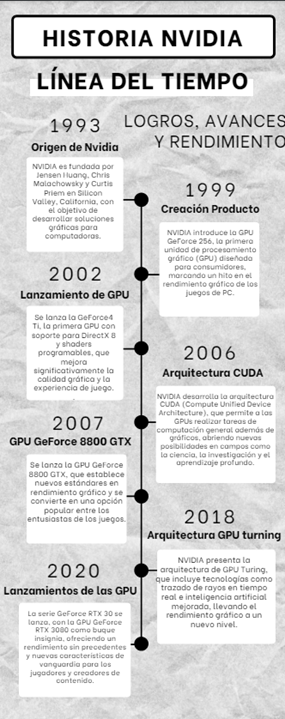
\includegraphics[width=\linewidth]{./Images/LineaTiempo.png}
		\caption{Linea de tiempo de NVIDIA}
	\end{center}
\end{figure}

\section{Objetivos y vision de la empresa}

La compañía NVIDIA Corporation es reconocida por ofrecer soluciones
en gráficos, computación y redes a nivel global. La oferta incluye
productos como las tarjetas gráficas GeForce, perfectas para
jugadores y usuarios de PC, y el servicio de transmisión de
juegos GeForce NOW.~Además, ofrecen soluciones para
profesionales, como las GPU Quadro/NVIDIA RTX, que se
utilizan en estaciones de trabajo para tareas gráficas
exigentes. También ofrecen una variedad de productos
para centros de datos y redes, como plataformas
informáticas y de redes, y se especializan en el área
de la conducción automatizada con su plataforma NVIDIA DRIVE.\@{}

Los videojuegos, la visualización profesional, los centros
de datos y la industria automotriz son algunos de los
principales sectores que se benefician de los productos de NVIDIA.~La
compañía vende sus productos a varios tipos de clientes,
como fabricantes de equipos originales, distribuidores y
proveedores de servicios en la nube.

\section{Marco Teorico}

\subsection*{Posicionamiento de NVIDIA en el mercado de tecnología y GPU}

\begin{itemize}
	\item Revisión de literatura sobre la evolución de NVIDIA
	      como líder en el mercado de procesamiento gráfico (GPU) y
	      tecnologías relacionadas.

	\item Análisis de las estrategias de marketing,
	      investigación y desarrollo que han contribuido al éxito de
	      NVIDIA en el mercado.

	\item Exploración de la relación entre la innovación
	      tecnológica, la calidad del producto y la percepción de la
	      marca en la posición competitiva de NVIDIA.\@{}
\end{itemize}

\subsection*{Mercados más y menos significativos para NVIDIA}

\begin{itemize}
	\item Identificación y análisis de los mercados verticales más
	      importantes para NVIDIA, como la inteligencia artificial, los
	      videojuegos, la computación en la nube, el automóvil autónomo
	      y la visualización profesional.

	\item Evaluación de oportunidades y desafíos en cada mercado,
	      incluyendo factores económicos, regulatorios y tecnológicos.

	\item Investigación de los mercados emergentes y nichos
	      de mercado que podrían ofrecer nuevas oportunidades de
	      crecimiento para NVIDIA, así como los mercados que pueden
	      estar disminuyendo en importancia.
\end{itemize}

\subsection*{Relación entre NVIDIA y el mercado Taiwanés}

\begin{itemize}
	\item Examen de la colaboración histórica entre NVIDIA y las
	      empresas taiwanesas en la fabricación de componentes
	      electrónicos, como chips de GPU y tarjetas gráficas.

	\item Análisis de la integración vertical y horizontal de la
	      cadena de suministro de NVIDIA en Taiwán, incluyendo
	      relaciones con fabricantes de semiconductores,
	      ensambladores de tarjetas gráficas y otros proveedores de
	      tecnología.

	\item Investigación de las políticas gubernamentales,
	      las condiciones económicas y las dinámicas empresariales en
	      Taiwán que pueden afectar la relación entre NVIDIA y el mercado
	      taiwanés.
\end{itemize}

\subsection*{Implicaciones para el futuro de NVIDIA}

\begin{itemize}
	\item Discusión de las oportunidades estratégicas y los riesgos
	      potenciales que enfrenta NVIDIA en el contexto de su posición
	      en el mercado y sus relaciones con Taiwán y otros mercados clave.

	\item Propuesta de recomendaciones para NVIDIA basadas en
	      las tendencias identificadas en la investigación, incluyendo
	      áreas de expansión, colaboración empresarial y gestión de riesgos.
\end{itemize}

\bibliography{./Bibliography/bibliography.bib}

\end{document}
